%%----------------------------------------------------------------------------
%% Presentatie HoGent Bedrijf en Organisatie
%%----------------------------------------------------------------------------
%% Auteur: Bert Van Vreckem [bert.vanvreckem@hogent.be]

\documentclass{beamer}

%==============================================================================
% Aanloop
%==============================================================================

%---------- Packages ----------------------------------------------------------

\usepackage{graphicx,multicol}
\usepackage{comment,enumerate,hyperref}
\usepackage{amsmath,amsfonts,amssymb}
\usepackage{tikz}
\usepackage{lmodern}
\usepackage[T1]{fontenc}
\usepackage[utf8]{inputenc}
\usepackage{csquotes}
\usepackage[dutch]{babel}
\usepackage{multirow}
\usepackage{eurosym}
\usepackage{listings}
\usepackage{textcomp}
\usepackage{framed}
\usepackage{wrapfig}
\usepackage[backend=biber,style=apa]{biblatex}
\DeclareLanguageMapping{dutch}{dutch-apa}
\addbibresource{onderzoekstechnieken_oef1.bib}

%---------- Configuratie ------------------------------------------------------

\usetikzlibrary{arrows,shapes,backgrounds,positioning,shadows}

\usetheme{hogent}

%---------- Commando-definities -----------------------------------------------

\newcommand{\tabitem}{~~\llap{\textbullet}~~}

%---------- Info over de presentatie ------------------------------------------

\title[Intro]{Onderzoekstechnieken\\Oefeningles 1. \LaTeX{}}
\author{Jens Buysse \and Wim {De Bruyn} \and Bert {Van Vreckem}}
\date{AJ 2017-2018}

%==============================================================================
% Inhoud presentatie
%==============================================================================

\begin{document}

%---------- Front matter ------------------------------------------------------

% Dia met het HoGent logo
\HoGentLogo

% Titeldia met faculteitslogo
\titleframe

%---------- Inhoud ------------------------------------------------------------

\begin{frame}
  \frametitle{What's on the menu today?}

  \tableofcontents
\end{frame}

\section{Inleiding}

\subsection{Filosofie, geschiedenis}

\begin{frame}
  \frametitle{Filosofie: waarom {\LaTeX}?}
  
  \begin{itemize}
  \item<+-> WYSIWYG tekstverwerkers dwingen auteurs om de vormgeving te verzorgen.
  \item<+-> Gevolg is slechte, inconsistente opmaak van documenten.
  \item<+-> Goede vormgeving van teksten is een \emph{specialisatie}, en wordt best
    uit handen van auteurs genomen.
  \item<+-> {\LaTeX} zorgt dat auteurs enkel over de \emph{inhoud} en \emph{structuur} van de tekst moet nadenken.
  \end{itemize}
\end{frame}

\begin{frame}
  \frametitle{Geschiedenis}

  \begin{columns}[c]

  \column{.67\textwidth}
    \begin{itemize}
    \item<+-> 1977: Donald Knuth vindt de drukproeven van zijn boek \emph{The art of Computer Programming} afschuwelijk
    \item<+-> 1978: Schreef dan maar zelf een tekstzetsysteem, {\TeX}
    \item<+-> 1989: Versie 3.0, sindsdien enkel bugfix-releases (convergeren naar $\pi$)
    \item<+-> 1980s: Leslie Lamport ontwikkelt markup-taal voor {\TeX}: {\LaTeX}
    \end{itemize}

  \column{.33\textwidth}
    \begin{center}
    \only<1-3>{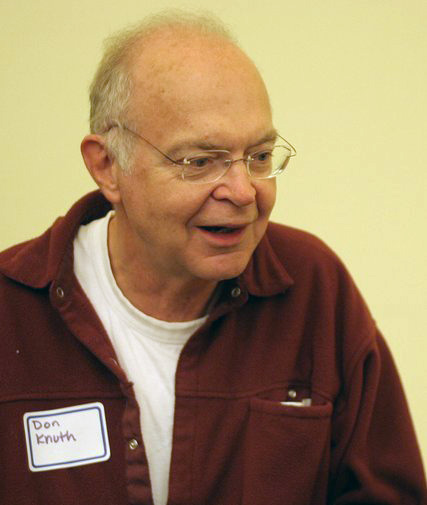
\includegraphics[width=\textwidth]{img/oef1-01}}
    \only<4->{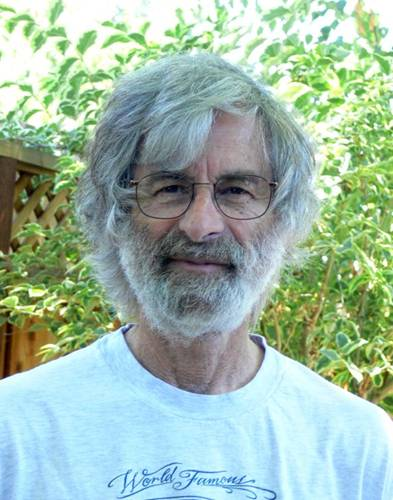
\includegraphics[width=\textwidth]{img/oef1-02}}
    \end{center}

  \end{columns}
\end{frame}

\subsection{Voorbeelden}

\begin{frame}
  \frametitle{Voorbeelden---papers}

  {\LaTeX} is de norm voor wetenschappelijke publicaties in computerwetenschappen, wiskunde, fysica, enz.

  \begin{center}
  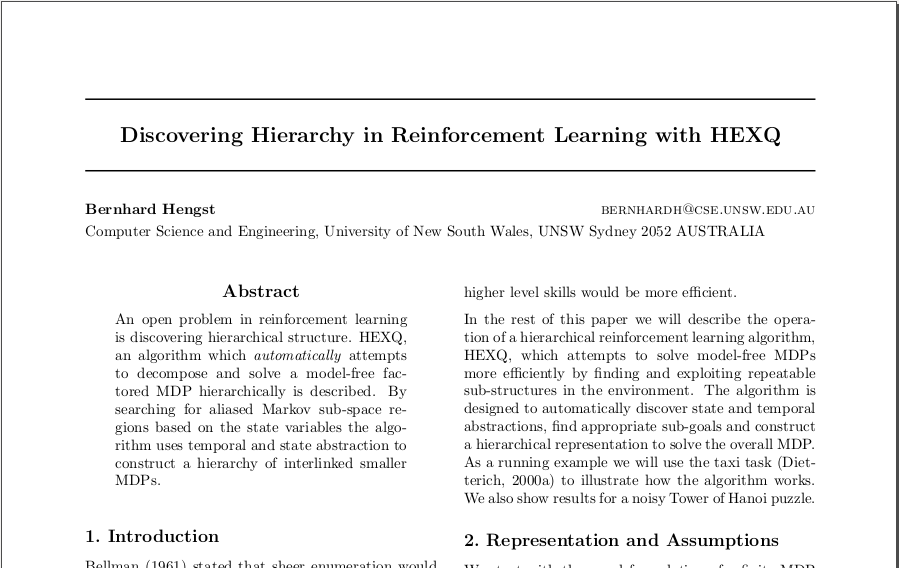
\includegraphics[height=.6\textheight]{img/oef1-03}
  \end{center}

\end{frame}

\begin{frame}
  \frametitle{Voorbeelden---boeken}

  Ook: cursussen, thesissen, enz.

  \begin{center}
	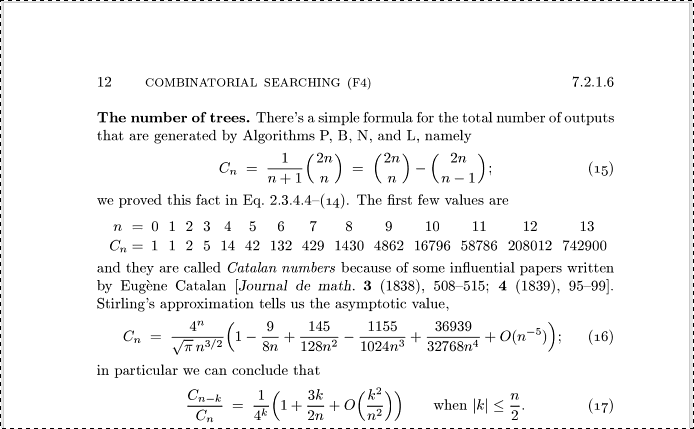
\includegraphics[height=.6\textheight]{img/oef1-04}
  \end{center}

\end{frame}

\begin{frame}
  \frametitle{Voorbeelden---presentaties}

  \begin{center}
  vb. deze presentatie\ldots
  \end{center}

\end{frame}

\begin{frame}
  \frametitle{Voordelen}

  \begin{itemize}
    \item<+-> Enkel bezighouden met inhoud, goede en consistente opmaak gegarandeerd.
    \item<+-> Tekstformaat $\Rightarrow$ geschikt voor versiebeheersysteem!
    \item<+-> Is de norm in verschillende onderzoeksdomeinen, o.a. computerwetenschappen
  \end{itemize}
\end{frame}


\begin{frame}
  \frametitle{Nadelen}

  \begin{itemize}
    \item<+-> Zware leercurve $\Rightarrow$ copy paste voorbeelden, gebruik infobronnen, vraag hulp
    \item<+-> Soms is gewenste opmaak niet makkelijk te bereiken (vb.~tabellen)
  \end{itemize}

  \uncover<1->{%
    \begin{center}
      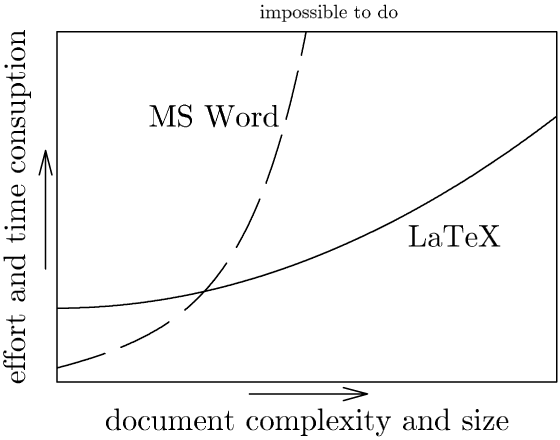
\includegraphics[height=.5\textheight]{img/oef1-05}
    \end{center}}
\end{frame}

\subsection{Hulp zoeken}

\begin{frame}
  \frametitle{Hulp zoeken}

  \begin{itemize}
  \item Tobias Oetiker, et al., \emph{The Not So Short Introduction to {\LaTeXe}}, 2011 (a.k.a. ``lshort'', versie 5.01)
  \item {\TeX} - {\LaTeX} StackExchange (Q \& A site): \url{http://tex.stackexchange.com/}
  \item \emph{{\LaTeX} Wikibook}, \url{http://en.wikibooks.org/wiki/LaTeX}
  \item \emph{Hypertext help with {\LaTeX}}, \url{http://www.ics.uci.edu/~pan/documents/latex/ltx-2.html}
  \end{itemize}

\end{frame}

\section{Aan de slag met {\LaTeX}}

\subsection{Werkomgeving opzetten}

\begin{frame}
  \frametitle{Werkomgeving opzetten}

(1) {\LaTeX} distributie
  
  \begin{itemize}
  \item Windows: MikTeX \url{http://miktex.org/}
  \item MacOS: MacTeX distribution \url{http://www.tug.org/mactex/2011/}
  \item Linux: zit in repositories
    \begin{itemize}
    \item Ubuntu, Debian: \texttt{sudo apt-get install texlive}
    \item Fedora: \texttt{sudo dnf install texlive}
    \end{itemize}
  \item On-line werkomgeving: \url{https://www.overleaf.com/}
  \end{itemize}

(2) {\LaTeX} editor

  \begin{itemize}
  \item Verschillende keuzes, afh.~besturingssysteem
  \item vb. TexStudio \url{http://www.texstudio.org/}
  \end{itemize}
\end{frame}

\subsection{Documentstructuur}

\begin{frame}
  \frametitle{Werkwijze}

  \begin{itemize}
  \item<+-> Schrijf tekst in {\LaTeX}\\
            = tekstbestand! (markuptaal zoals HTML)
  \item<+-> Compileer met \texttt{pdflatex} (evt. verschillende keren)
  \item<+-> Bekijk resultaat in PDF
  \end{itemize}
\end{frame}

\begin{frame}[fragile]
  \frametitle{{\LaTeX} commando's}

  \begin{block}{Basis-syntax}
  \verb|\commandonaam[optionele,argumenten]{arg1}{arg2}|
  \end{block}

  \pause

  Bijvoorbeeld:

  \begin{itemize}
  \item<+-> \verb|\documentclass[a4paper,pdftex,12pt]{paper}|
  \item<+-> \verb|\'{e}l\`{e}ve| $\Rightarrow$ \'el\`eve
  \item<+-> \verb|\begin{itemize}|\\
            \verb|\item lijst|\\
            \verb|\end{itemize}|
  \end{itemize}

\end{frame}

\begin{frame}[fragile]
  \frametitle{Een document opbouwen}
  
  \begin{center}
  \alert{%
  \only<1>{Definitie documentsoort (hier: artikel)}
  \only<2>{``body'' van het document}
  \only<3>{Documentinhoud}
  \only<4>{Extra functionaliteit beschikbaar maken}
  \only<5>{Titel, auteur komt in ``preamble''}
  \only<6>{Titel in document invoegen}
  }
  \end{center}

\begin{semiverbatim}
\uncover<1->{\alert<1>{\\documentclass[a4paper,12pt]\{article\}}}
\uncover<4->{\alert<4>{\\usepackage[dutch]\{babel\}}}
\uncover<5->{\alert<5>{\\title\{Minimaal \{\\LaTeX\} document\}}}
\uncover<5->{\alert<5>{\\author\{Bert \{Van Vreckem\}\}}}
\uncover<5->{\alert<5>{\\date\{\\today\}}}
\uncover<2->{\alert<2>{\\begin\{document\}}}
\uncover<6->{\alert<6>{\\maketitle}}
\uncover<3->{\alert<3>{Lorem ipsum dolor sit amet, consectetur adipiscing elit.}}
\uncover<2->{\alert<2>{\\end\{document\}}}
\end{semiverbatim}

\end{frame}

\begin{frame}
  \frametitle{Resultaat}
  
  \begin{center}
  
\includegraphics[height=.6\textheight]{img/oef1-06}
  \end{center}
\end{frame}

\begin{frame}[fragile]
  \frametitle{Documenttypes}
  
  \begin{center}
  \begin{semiverbatim}
  \\documentclass[\alert<2>{OPTIONS}]\{\alert<1>{TYPE}\}
  \end{semiverbatim}
  \end{center}

\only<1>{%  
  \begin{center}
  \begin{tabular}{ll}
    \hline
    TYPE & soort document \\
    \hline
    \texttt{article} & artikel, paper, korte tekst \\
    \texttt{beamer} & presentatie \\
    \texttt{book} & boek \\
    \texttt{report} & (lang) rapport, thesis, verslag, \ldots \\
  \end{tabular}
  \end{center}
}
\only<2>{%  
  \begin{center}
  \begin{tabular}{ll}
    \hline
    OPTION & soort document \\
    \hline
    \texttt{12pt} & 12-puntsletters (ipv 10pt) \\
    \texttt{a4paper} & A4 (ipv Am. Letter) \\
    \texttt{twocolumn} & gebruikelijk bij artikels \\
    \texttt{twoside} & voor dubbelzijdig afdrukken \\
  \end{tabular}
  \end{center}
}
\end{frame}



\begin{frame}[fragile]
  \frametitle{Documentstructuur}
  
  \begin{center}
  \begin{tabular}{ll}
    \verb?\part? & (geen invloed op hoofdstuknummers) \\
    \verb?\chapter? & (enkel in \texttt{book}, \texttt{report}) \\
    \verb?\section? & \\
    \verb?\subsection? & \\
    \verb?\subsubsection? & (niet in \texttt{book}, \texttt{report}) \\ 
    \verb?\paragraph? & \\
    \verb?\subparagraph? & \\
    &\\
    \verb?\appendix? & vanaf hier wordt \verb?\chapter? een Bijlage \\
    \verb?\label{?\texttt{\ldots}\verb?}? & voor verwijzingen (met \verb|\ref{LABEL}|)
  \end{tabular}
  \end{center}
\end{frame}

\begin{frame}[fragile]
  \frametitle{Preamble---Nuttige packages}
  
  \begin{description}
  \item[\texttt{\textbackslash{}usepackage\{amsfonts\}}] AMS math packages: extra wiskundige
  \item[\texttt{\textbackslash{}usepackage\{amsmath\}}] symbolen (o.a. getallenverzamelingen
  \item[\texttt{\textbackslash{}usepackage\{amssymb\}}] $\mathbb{N}, \mathbb{R}, \mathbb{Z}, \mathbb{Q}$, etc.)
  \pause
  \item[\texttt{\textbackslash{}usepackage[dutch]\{babel\}}] Taalinstellingen: woordsplitsingen, commando's voor speciale karakters ("dutch" voor NL)
  \pause
  \item[\texttt{\textbackslash{}usepackage\{eurosym\}}] Euro-symbool (\euro)
  \pause
  \item[\texttt{\textbackslash{}usepackage\{fancyhdr\}}] Pagina-opmaak met hoofd- en voettekst
  \pause
  \item[\texttt{\textbackslash{}usepackage\{graphicx\}}] Invoegen van figuren
  \end{description}
\end{frame}

\begin{frame}[fragile]
  \frametitle{Preamble---Nuttige packages}
  
  \begin{description}
  \item[\texttt{\textbackslash{}usepackage[pdftex,bookmarks=true]\{hyperref\}}] PDF krijgt klikbare links \& verwijzingen, inhoudstafel \pause
  \item[\texttt{\textbackslash{}usepackage[utf8]\{inputenc\}}] Accenten gebruiken in tekst (vb. é ipv \verb|\'e|) \pause
  \item[\texttt{\textbackslash{}usepackage\{listings\}}] Broncode mooi opmaken \pause
  \item[\texttt{\textbackslash{}usepackage\{multirow\}}] Tekst over verschillende cellen in tabellen \pause
  \item[\texttt{\textbackslash{}usepackage\{rotating\}}] Tabellen en figuren roteren \pause
  \item[\texttt{\textbackslash{}usepackage\{lipsum\}}] Vultekst (lorem ipsum dolor sit amet\ldots)
  \end{description}
\end{frame}

\subsection{Tekst schrijven}

\begin{frame}[fragile]
  \frametitle{Tekstopmaak}
  
  \begin{itemize}
  \item<+-> Speciale tekens ({\LaTeX} syntax): \% \$ \& \{ \} \textbackslash{} enz: \\
\begin{semiverbatim}
\\\% \\\$ \\\& \\\{ \\\} \\textbackslash\{\}
\end{semiverbatim}
  \item<+-> Ligaturen: \textrm{fi fl ffi ffl} (automatisch opgemaakt)
  \item<+-> Accenten: \'{e} \`{e} \^{e} \"{e} \={e} \c{c} enz.
\begin{semiverbatim}
\\'\{e\} \\`\{e\} \\^\{e\} \\"\{e\} \\=\{e\} \\c\{c\} enz.
\end{semiverbatim}
  \item<+-> Ellipsis (\ldots): \texttt{\textbackslash{}ldots}
  \item<+-> Aanhalingstekens: `enkel' ``dubbel''
\begin{verbatim}
`enkel' ``dubbel''
\end{verbatim}
  \end{itemize}
\end{frame}

\begin{frame}[fragile]
  \frametitle{Letterstijlen}
  
  \begin{center}
  \begin{tabular}{ll}
    \hline
    Commando & resultaat \\
    \hline
    \verb?\emph{xxx}?   & \emph{Benadrukken} (\textrm{\emph{cursief}} of \textsf{\emph{`slanted'}})\\
    \verb?\textit{xxx}? & \textit{Cursieve tekst} \\
    \verb?\textbf{xxx}? & \textbf{Vetgedrukte tekst} \\    
    \verb?\texttt{xxx}? & \texttt{Monogespatieerde letters} \\
    \verb?\textrm{xxx}? & \textrm{Schreefletters}  \\
    \verb?\textsf{xxx}? & \textsf{Schreefloze letters}  \\
    \verb?\textsc{xxx}? & \textsc{Small Caps} \\
  \end{tabular}
  \end{center}

\end{frame}

\begin{frame}[fragile]
  \frametitle{Lijstomgevingen}
  
  \begin{columns}[c]
  \column{.49\textwidth}
\begin{verbatim}  
\begin{itemize}
\item Een onderdeel
\item Nog een onderdeel
\end{itemize}
\end{verbatim}

  \column{.49\textwidth}
\begin{itemize}
\item Een onderdeel
\item Nog een onderdeel
\end{itemize}
  \end{columns}

\pause

  \begin{columns}[c]
  \column{.49\textwidth}
\begin{verbatim}  
\begin{enumerate}
\item Een onderdeel
  \begin{enumerate}
  \item extra niveau
  \end{enumerate}
\item Nog een onderdeel
\end{enumerate}
\end{verbatim}

  \column{.49\textwidth}
\begin{enumerate}
\item Een onderdeel
  \begin{enumerate}
  \item extra niveau
  \end{enumerate}
\item Nog een onderdeel
\end{enumerate}
  \end{columns}

\end{frame}

\section{Figuren, tabellen, enz. invoegen}

\subsection{Figuren}

\begin{frame}[fragile]
  \frametitle{Figuren invoegen}

  \begin{columns}[c]
  \column{.65\textwidth}
\begin{semiverbatim}
\alert<1>{\\begin\{figure\}}
  \alert<2>{\\includegraphics[width=\\textwidth]
    \{img/oef1-01\}}
  \alert<3>{\\caption\{Donald Knuth, auteur van
    \{\\TeX\}\}}
  \alert<4>{\\label\{fig:don\}}
\alert<1>{\\end\{figure\}}
\end{semiverbatim}

  \column{.35\textwidth}
    \begin{figure}
      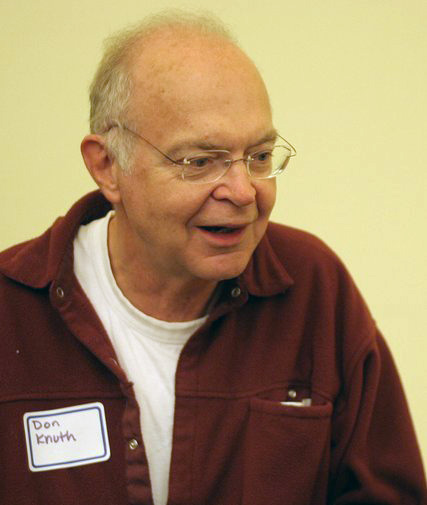
\includegraphics[width=\textwidth]{img/oef1-01}
      \caption{Donald Knuth, auteur van {\TeX}}
      \label{fig:don}
    \end{figure}

  \end{columns}

\end{frame}

\subsection{Tabellen}

\begin{frame}[fragile]
  \frametitle{Tabellen invoegen}
  
 \begin{columns}[c]
  \column{.6\textwidth}
  \small
\begin{semiverbatim}
\alert<1>{\\begin\{table\}}
  \alert<3>{\\begin\{tabular\}\{\alert<4>{l||c|r}\}}
  \alert<4>{\\hline}
  cel11 \alert<5>{&} 
    \alert<7>{\\multicolumn\{2\}\{c\}\{cel12\}} \alert<6>{\\\\}
  \alert<4>{\\hline \\hline}
  cel21 \alert<5>{&} cel22 \alert<5>{&} 
    \alert<7>{\\multirow\{2\}\{*\}\{cel23\}} \alert<6>{\\\\}
  cel31 \alert<5>{&} cel32 \alert<5>{&} \alert<6>{\\\\}
  \alert<3>{\\end\{tabular\}}
  \alert<2>{\\caption\{Een voorbeeldje van 
    wat je met tabellen kan doen\}
  \\label\{tab:vb_tabel\}}
\alert<1>{\\end\{table\}}
\end{semiverbatim}

  \column{.4\textwidth}
    \begin{table}
      \begin{tabular}{l||c|r}
      \hline
      cel11 & \multicolumn{2}{c}{cel12} \\
      \hline \hline
      cel21 & cel22 & \multirow{2}{*}{cel23} \\
      cel31 & cel32 & \\
      \end{tabular}
      \caption{Een voorbeeldje van wat je met tabellen kan doen}
      \label{tab:vb_tabel}
    \end{table}
  
  \end{columns}
\end{frame}

\subsection{Broncode}

\begin{frame}[fragile]
  \frametitle{Broncode invoegen: simpel}

\begin{semiverbatim}
\alert{\\begin\{verbatim\}}
public class MyApp \{
  public static void main(String args[]) \{
    System.out.println("Hello World");
  \}
\}
\alert{\\end\{verbatim\}}
\end{semiverbatim}
$\Rightarrow$
\begin{verbatim}
public class MyApp {
  public static void main(String args[]) {
    System.out.println("Hello World");
  }
}
\end{verbatim}  

\end{frame}

\begin{frame}[fragile]
  \frametitle{Broncode invoegen: \texttt{\textbackslash{}usepackage\{listings\}}}

\begin{semiverbatim}
\\lstset\{\%
  language=java,    breaklines=true,
  numbers=left,     frame=single,
  caption=\{Mijn eerste Java-programma.\},
  label=code:helloworld
\}

\alert{\\begin\{lstlisting\}}
public class MyApp \{
  public static void main(String args[]) \{
    System.out.println("Hello World");
  \}
\}
\alert{\\end\{lstlisting\}}
\end{semiverbatim}

\end{frame}

\begin{frame}[fragile]
  \frametitle{Broncode invoegen:  \texttt{\textbackslash{}usepackage\{listings\}}}

  \lstset{%
  language=java,    breaklines=true,
  numbers=left,     frame=single,
  caption={Mijn eerste Java-programma.},
  label=code:helloworld
}

\begin{lstlisting}
public class MyApp {
  public static void main(String args[]) {
    System.out.println("Hello World");
  }
}
\end{lstlisting}

\end{frame}

\subsection{Literatuurlijst}

\begin{frame}[fragile]
  \frametitle{Literatuurlijst}
  
  \begin{itemize}
  \item<+-> Literatuurlijst is belangrijk onderdeel van een thesis
  \item<+-> Strakke regels voor opmaak (HoGent: APA-stijl)
  \item<+-> Enkel \emph{publicaties} komen in aanmerking
  \item<+-> Enkel werken waarnaar verwezen wordt in de tekst
  \item<+-> {\LaTeX}, meer bepaald Bib{\LaTeX} helpt:
    \begin{itemize}
    \item<+-> ``bibliografische databank'' (in tekstformaat)
    \item<+-> Automatische opmaak, sortering literatuurlijst
    \item<+-> Verwijzingen vanuit uit de tekst (\verb|\textcite{}|)
    \item<+-> Ondersteuning via externe tools (e.g. JabRef, Mendeley Desktop)
    \end{itemize} 
  \end{itemize}
\end{frame}

\begin{frame}[fragile]
  \frametitle{Literatuurlijst}

Voorbeeld inhoud Bib{\LaTeX}-bestand (*.bib):

\begin{semiverbatim}
\alert<2>{@book}\{\alert<4>{Knuth1998},
 \alert<3>{author} = \{Knuth, Donald E.\},
 \alert<3>{title} = \{The art of computer programming,  volume 3:
   sorting and searching\},
 \alert<3>{year} = \{1998\},
 publisher = \{Addison Wesley\},
 address = \{Redwood City, CA, USA\}
\} 
\end{semiverbatim}

\only<2>{Of: article, inproceedings, inbook, phdthesis, misc, \ldots}
\only<3>{Sommige velden verplicht, afh. type publicatie}
\only<4>{Verwijzing in de tekst: 
  \begin{itemize}
     \item \alert{\texttt{\textbackslash{}textcite\{Knuth1998\}}} $\Rightarrow$ \textcite{Knuth1998}
    \item \alert{\texttt{\textbackslash{}autocite\{Knuth1998\}}} $\Rightarrow$ \autocite{Knuth1998}
  \end{itemize}
}

\end{frame}

\begin{frame}[fragile]
  \frametitle{Literatuurlijst}

Bibliografie invoegen:
\begin{semiverbatim}
\\usepackage[backend=bibtex,style=apa]\{biblatex\} \% Preamble
\\DeclareLanguageMapping\{dutch\}\{dutch-apa\}
\\addbibresource\{<database>\}
\dots
Verwijzingen in de tekst~\\textcite\{label\}.
\ldots
\\printbibliography
\end{semiverbatim}

$\Rightarrow$

\printbibliography

\end{frame}

\begin{frame}
  \frametitle{Literatuurlijst}

  Korte teksten: genummerd, volgens voorkomen (e.g. article)
  \begin{center}
  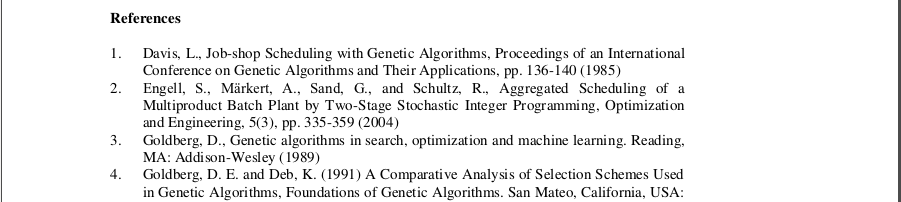
\includegraphics[width=.7\textwidth]{img/oef1-07}
  \end{center}

  Langere teksten: namen, alfabetisch (e.g. report, book)
  \begin{center}
  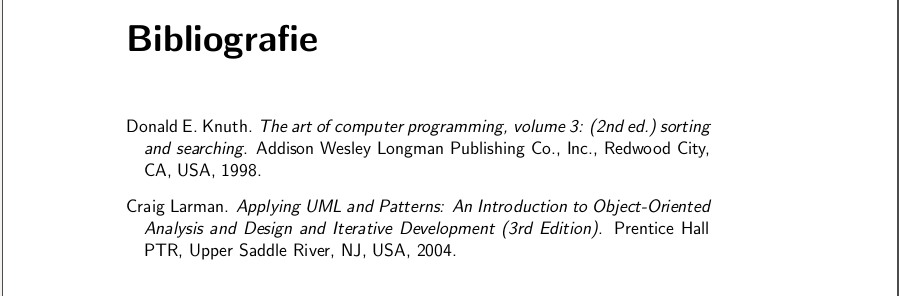
\includegraphics[width=.7\textwidth]{img/oef1-08}
  \end{center}

  \brightbox{HoGent gebruikt de ``APA''-stijl voor de opmaak van bibliografieën \url{https://bib.hogent.be/how-to/bronnen-vermelden/refereren-volgens-apa6th/}}

\end{frame}

\section{Tot slot}

\begin{frame}
  \frametitle{Tot slot}
  
  \begin{itemize}
  \item Een heleboel niet besproken:
    \begin{itemize}
    \item<+-> Wiskundige formules, vb.
    \begin{semiverbatim}
    \$x=-\\frac\{b \\pm \\sqrt\{b\^{}2 - 4ac\}\}\{2a\}\$
    \end{semiverbatim}
    $x=-\frac{b \pm \sqrt{b^2 - 4ac}}{2a}$
    \item<+-> Honderden packages (RTFM, Google is your friend)
    \item<+-> Presentaties met Beamer (baseer je bv. op het sjabloon op \url{https://bitbucket.org/bertvanvreckem/hogent-latex-sjablonen}

    \end{itemize}
  \item<+-> Hulp nodig? Na googlen, contacteer gerust \texttt{bert.vanvreckem@hogent.be}, \texttt{jens.buysse@hogent.be}
  \end{itemize}
\end{frame}

\end{document}
